A \emph{risk }is a potential condition that can lead to a the loss
of some value, either resource (economic or not) or time. \emph{Risk
Mitigation, Monitoring, and Management} (\emph{RMMM}) is a key step
of any project plan, it is intended to help to pre-determine any possible
major risks that may occur during development of this software. In
this section we will identify the main risks concerning the development
of myTaxiService and we will propose some strategy to tackle them.


\subsection{Introduction}

In this section we provide an analysis of the main risks harming the
myTaxiService project. For each risk identified we will provide the
the corresponding category \emph{project risks},\emph{ technical risks
}and\emph{ business risks, }an estimation of the probability and the
impact on the project %
\footnote{Probability and impact are expressed according to the standard qualitative
scale. For probability: Certain, Likely, Possible, Unlikely, Rare.
For impact/effect: Negligible, Marginal, Critical, Catastrophic.%
}.


\subsubsection{Project risks}

\emph{Project risks} (also known as development risks) are risks that
might threaten the project plan, if one of them becomes real it will
harm the project schedule, making it slip and increase the overall
cost. In myTaxiService we identified the following project risks.

\medskip{}


\begin{tabular}{>{\raggedright}p{4cm}|>{\raggedright}p{5cm}|>{\centering}p{2cm}|>{\centering}p{2cm}}
\hline 
\emph{Name} & \emph{Description} & \emph{Probability} & \emph{Impact}\tabularnewline
\hline 
\hline 
\emph{Requirement problem - 1} & Requirement engineers misunderstood the the requirements. & Possible & Catastrophic\tabularnewline
\hline 
\emph{Requirement problem - 2} & Customers changes the requirement in the late phases of the software
development. & Possible & Catastrophic\tabularnewline
\hline 
\emph{Requirement problem - 3} & The customer is not available when needed & Likely & Marginal\tabularnewline
\hline 
\emph{Personnel problem - 1} & Project manager is absent at critical times in the project. & Unlikely & Critical\tabularnewline
\hline 
\emph{Personnel problem - 2} & Some team members are absent at the critical times in the project. & Unlikely & Marginal\tabularnewline
\hline 
\emph{Personnel problem - 3} & Development team is not qulified to program a complex application
with JEE. & Likely & Critical\tabularnewline
\hline 
\emph{Personnel problem - 4} & Miscommunication in the project team. & Possible & Critical\tabularnewline
\hline 
\emph{Personnel problem - 5} & Lack of documentation. & Rare & Critical\tabularnewline
\hline 
\end{tabular}


\subsubsection{Business risks}

\emph{Business risks} can threaten the viability of the software to
be produced; if one of them becomes real it can compromise the economic
success of the project. In myTaxiService system we identified the
following business risks.

\medskip{}


\begin{tabular}{>{\raggedright}p{4cm}|>{\raggedright}p{5cm}|>{\centering}p{2cm}|>{\centering}p{2cm}}
\hline 
\emph{Name} & \emph{Description} & \emph{Probability} & \emph{Impact}\tabularnewline
\hline 
\hline 
\emph{Market risk} & There is no demand for product, passengers prefer to use the traditional
channels to call for a taxi. & Possible & Catastrophic\tabularnewline
\hline 
\emph{Budget risk} & Due to organizational financial problems the budget is reduced. & Unlikely & Catastrophic\tabularnewline
\hline 
\end{tabular}


\subsubsection{Technical risks}

\emph{Technical risks} can threaten the quality and the timeliness
of the software to be developed; if a technical risk becomes real
it can make the implementation more difficult or even impossible.
In myTaxiService system we identified the following technical risks.

\medskip{}


\begin{tabular}{>{\raggedright}p{4cm}|>{\raggedright}p{5cm}|>{\centering}p{2cm}|>{\centering}p{2cm}}
\hline 
\emph{Name} & \emph{Description} & \emph{Probability} & \emph{Impact}\tabularnewline
\hline 
\hline 
\emph{Design problem - 1} & The architectural style and patter chosen in the architectural design
phase are not suitable for the kind of application to be developed. & Unlikely & Catastrophic\tabularnewline
\hline 
\emph{Design problem - 2} & The algorithm for taxi management proposed in the design phase are
not correct.  & Rare & Serious\tabularnewline
\hline 
\emph{Design problem - 3} & Design does not reflect requirements & Unlikely & Catastrophic\tabularnewline
\hline 
\emph{Implementation problem - 1} & Poor comments in the code. & Possible & Marginal\tabularnewline
\hline 
\emph{Implementation problems - 2} & Code does not follow quality guidelines. & Unlikely & Critical\tabularnewline
\hline 
\emph{Implementation problem - 3} & The code does not reflect the designed architecture. & Unlikely & Critical\tabularnewline
\hline 
\emph{Performance problems - 1} & The DBMS cannot meet the performance requirements.  & Unlikely & Catastrophic\tabularnewline
\hline 
\end{tabular}


\subsection{Risk strategy}

A \emph{risk strategy} defines a set of rules to be applied in order
to manage and tackle risk. Those strategies are typically divided
into:
\begin{itemize}
\item \emph{Reactive risk strategies}: there is no explicit risk management,
nothing is done about risk until something goes wrong. This is the
typical approach that is adopted by the majority of software teams
and managers. This strategy is also known as \emph{crisis management}
since no preventive measure is designed.
\item \emph{Proactive risk strategies}: risk identification, analysis and
ranking are performed in advance in order to develop a \emph{contingency}
plan to manage risk having high probability and high impact. This
approach, even if more costly, is aimed to avoid risk in order to
be able to deal with only unforeseen risks.
\end{itemize}
Since in the previous section we have identified the risks, we are
actually following the proactive risk strategy. We think that identifying
the risks, set up proper measures in order to tackle them in an appropriate
way would make smaller the economic effort in the future stages.

\begin{figure}[H]
\noindent \begin{centering}
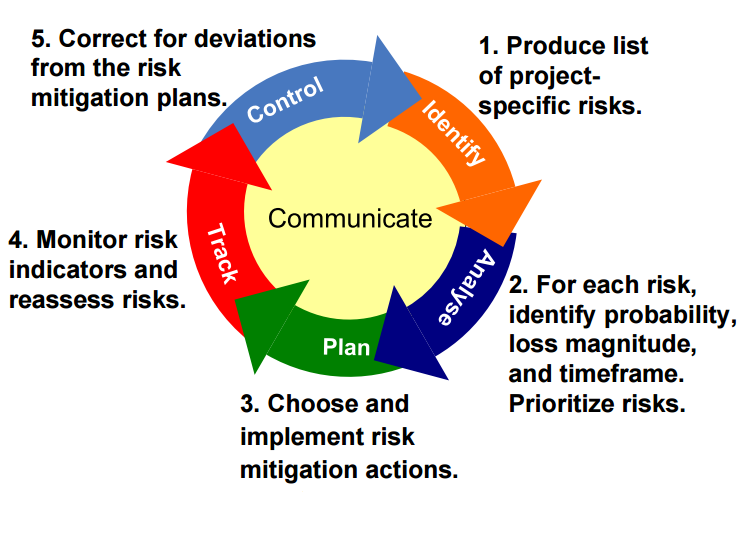
\includegraphics[scale=0.75]{risks/images/risk}
\par\end{centering}

\protect\caption{Proactive risk strategy cycle}
\end{figure}


In the following tables we report for each risk identified in the
previous section a possible \emph{prevention plan} or a \emph{correction
plan}.

\begin{landscape}


\subsubsection{Project risks}

\medskip{}


\begin{tabular}{>{\raggedright}p{4cm}|>{\raggedright}p{10cm}|>{\raggedright}p{8cm}}
\hline 
\emph{Name} & \emph{Prevention} & \emph{Correction}\tabularnewline
\hline 
\hline 
\emph{Requirement problem - 1} & \begin{itemize}
\item {\small{}Adopt a formalized method for requirement engineering (like
Jackson-Zave approach).}{\small \par}
\item {\small{}Perform validation of requirements right before design phase
by meeting the stakeholders.}{\small \par}
\item {\small{}After requirement engineering phase provide customers with
a small prototype.}\end{itemize}
 & {\small{}Recycle on the requirement engineering phase fixing the RASD.}\tabularnewline
\hline 
\emph{Requirement problem - 2} & \begin{itemize}
\item {\small{}It is explained to the customer, that after he has accepted
a version of the RASD, it cannot be changed by the customer’s wish
only.}{\small \par}
\item {\small{}Trace the requirements in order to quantify the effort of
changing.}\end{itemize}
 & {\small{}Recycle on the requirement engineering phase fixing the RASD.}\tabularnewline
\hline 
\emph{Requirement problem - 3} & \begin{itemize}
\item {\small{}Try to stay in touch with the customer in order to increase
his interest on the product.}{\small \par}
\item {\small{}Meetings with the customer can be planned well in advance.}\end{itemize}
 & {\small{}When the customer is not available, meetings may have to
be rescheduled. }\tabularnewline
\hline 
\emph{Personnel problem - 1} & {\small{}Nominate a vice project manager.} & {\small{}Vice project manager takes over the role of the project manager.}\tabularnewline
\hline 
\emph{Personnel problem - 2} & \begin{itemize}
\item {\small{}Team members should warn the project manager timely before
a planned period of absence.}{\small \par}
\item {\small{}Ensure that knowledge is shared between team members}\end{itemize}
 & {\small{}An other team member takes care of the work.}\tabularnewline
\hline 
\end{tabular}

\begin{tabular}{>{\raggedright}p{4cm}|>{\raggedright}p{10cm}|>{\raggedright}p{8cm}}
\hline 
\emph{Name} & \emph{Prevention} & \emph{Correction}\tabularnewline
\hline 
\hline 
\emph{Personnel problem - 3} & {\small{}Provide an introductory course to JEE} & \tabularnewline
\hline 
\emph{Personnel problem - 4} & \begin{itemize}
\item {\small{}After a meeting, one group member creates an interview report. }{\small \par}
\item {\small{}Team members should not hesitate to ask and re-ask questions
if things are unclear.}\end{itemize}
 & {\small{}When it becomes clear that miscommunication is causing problems,
the team members involved and the customer are gathered in a meeting
to clear things up.}\tabularnewline
\hline 
\emph{Personnel problem - 5} & {\small{}Impose that before starting a new phase of the software development
the corresponding document is ready.} & {\small{}Ask the employee to write documentation.}\tabularnewline
\hline 
\end{tabular}

\medskip{}



\subsubsection{Business risks}

\medskip{}


\begin{tabular}{>{\raggedright}p{4cm}|>{\raggedright}p{10cm}|>{\raggedright}p{8cm}}
\hline 
\emph{Name} & \emph{Prevention} & \emph{Correction}\tabularnewline
\hline 
\hline 
\emph{Market risk} & {\small{}Make sure there is the interest around the product.} & {\small{}Advertise the product.}\tabularnewline
\hline 
\emph{Budget risk} & {\small{}Make sure at the beginning of the project that there is the
availability of budget.} & {\small{}Communicate with the founders showing how the project makes
a contribution to the goals of the business and argument about the
fact that cuts to the budget would not be cost effective.}\tabularnewline
\hline 
\end{tabular}

\newpage{}


\subsubsection{Technical risks}

\medskip{}


\begin{tabular}{>{\raggedright}p{4cm}|>{\raggedright}p{10cm}|>{\raggedright}p{8cm}}
\hline 
\emph{Name} & \emph{Prevention} & \emph{Correction}\tabularnewline
\hline 
\hline 
\emph{Design problem - 1} & \begin{itemize}
\item {\small{}Perform inspection of the DD.}{\small \par}
\item {\small{}Ask some advisor on his opinion about the feasibility and
the correctness of certain design decisions.}\end{itemize}
 & \begin{itemize}
\item {\small{}When errors in the design are noticed consulted some advisor
to help correct the design errors as soon as possible. }{\small \par}
\item {\small{}Also all the work, that depends on the faulty design, should
be halted until the error is corrected.}\end{itemize}
\tabularnewline
\hline 
\emph{Design problem - 2} & {\small{}Use simulation techniques to test the correctness of the
algorithm} & {\small{}Revise the algorithm in order to fix the flaws.}\tabularnewline
\hline 
\emph{Design problem - 3} & \begin{itemize}
\item {\small{}Perform inspection of the DD.}{\small \par}
\item {\small{}Show at least some part of the DD to the customer in order
to see his/her opinion.}\end{itemize}
 & {\small{}Recycle on the design phase fixing the DD.}\tabularnewline
\hline 
\emph{Implementation problem - 1} & {\small{}Provide the developer with a clear specification of what
to comment.} & {\small{}Ask the developer to add the missing comments.}\tabularnewline
\hline 
\emph{Implementation problems - 2} & \begin{itemize}
\item {\small{}Provide the developer with a document in which code conventions
are stated.}{\small \par}
\item {\small{}Perform code inspection.}\end{itemize}
 & {\small{}Ask the developer to fix the issues.}\tabularnewline
\hline 
\emph{Implementation problem - 3} & \begin{itemize}
\item {\small{}Perform unit testing after each module is ready}{\small \par}
\item {\small{}Continuesly check the work of the developers}\end{itemize}
 & {\small{}Ask the developer to fix the involved component.}\tabularnewline
\hline 
\emph{Performance problems - 1} & {\small{}Estimate the load and acquire a suitable DBMS.} & {\small{}Investigate the possibility of acquiring a highier performance
DBMS.}\tabularnewline
\hline 
\end{tabular}

\end{landscape}
